\chapter{Introduction\label{chap:introduction}}
\section{Motivation}
% Drug discovery is important. 
Drug discovery is the process of identifying new medicines and bringing them to
market. The discovery of novel pharmaceutical treatments has been a major driver
of quality of life over the centuries. While discovery of new drugs has started 
in serendipitous and lucky discoveries, advances in science and technology  
led to an ever more systematic and data-driven approach, especially over the
last decades. 

% Traditional way of finding candidates.
One of the key challenges of the drug discovery process is the identification
of novel promising drug candidates. The efficacy of a drug is usually determined by its ability
to interact with a biological target in the body. To find such molecules,
the traditional approach is to synthesize and test the molecules efficacy first in laboratory
experiments, and finally in clinical studies. However, this process is usually very expensive, time-consuming
and can involve risks for patients.

% Computer aided drug discovery
Computer aided drug discovery (CADD) aims to accelerate the drug discovery
process using computational methods. Applications range from basic chemical
information processing, over physical simulation of molecular interactions, to
sophisticated machine learning methods. Advances in deep learning
\citep{chenRiseDeepLearning2018} have led to breakthroughs in many different
areas of drug discovery, including highly accurate protein structure prediction 
achieved by AlphaFold \citep{todo}, chemical property prediction
\citep{mayrDeepToxToxicityPrediction2016,todo}, synthesis planning
\citep{seglerNeuralSymbolicMachineLearning2017} and molecule generation
\citep{todo}. These advances help by reducing the need for expensive 
wet-lab experiments and can assist chemists in drug design tasks. 

% Significance and objectives of the thesis
In this thesis, we focus on two key areas where machine learning can help to
accelerate the drug discovery process: generative models for molecules and
computer-aided synthesis planning (CASP). Generative models have been shown to
be able to efficiently find molecular structures satisfying property profiles of
interest, and have been used to generate novel drug candidates. However, the
evaluation of generative models is challenging, as the outputs of these models
are usually complex, structured objects, and there are often no straightforward
ways to evaluate the quality or relevance of the generated molecules. In this
thesis, we address this issue by proposing new evaluation metrics and benchmarks
for generative models.

% CASP
Computer-aided synthesis planning (CASP) assists chemists in the task of
synthesizing target molecules. CASP tools are based on a combination of planning
algorithms and computational chemical reaction models, and suggest synthesis
plans for molecules of interest. Highly accurate chemical reaction models are
necessary for satisfactory performance of CASP tools. Many such models are based
on reaction templates, which encode the connectivity changes between atoms that
occur during a chemical reaction. In this thesis we propose a novel
template-based reaction model for the problem of single-step retrosynthesis
prediction \citep{todo}. 

% PROMISE
This thesis is structured as follows. In \cref{sec:generative-models} we give 
an overview of generative models for molecules, discuss the challenges of evaluating
these models and present our contributions to this field. In \cref{sec:retrosynthesis}
we give a short overview of computer-aided synthesis planning and outline our contributions. 
\Cref{sec:publications} lists the publications that are part of this thesis and 
related publications. \Cref{chap:publications} reprints the publications
and their corresponding supplementary material. Finally, \cref{chap:conclusion} concludes
the thesis and gives an outlook on future work.



% \begin{minipage}
% : Rational drug discovery.
% This approach starts with the identification of a biological target in the body 
% which is hypothesized to be associated with a disease phenotype. 
% One then attempts to find a small molecule that can change the activity of 
% the target in the desired way. While this way of searching for new drugs 
% is more direct than phenotypic drug discovery the identification of 
% drug targets can be challenging and given the complex interconnectedness 
% of biochemical pathways, it is not fully understood how some drugs work, 
% which goes even for highly popular ones.

% Phenotypic drug discovery takes this trial-and-error approach and applies it 
% in a systematic manner. The focus in this approach, which is also called forward 
% pharmacology, lies on screening collections of small molecules or other potential 
% medicines for pharmaceutical effects. Once a pharmacologically active molecule 
% has been found the aim is to discover how to use it's effect therapeutically. 
% This process can proceed without knowing the biochemical mode of action, of how 
% a drug actually achieves its effect. 

% How were new medicines discovered?
% David C. Swinney & Jason Anthony 
% Lots of molecules also by phenotypic screening

% One of core goals in both approaches is to find molecules with a desired
% pharmacological profile, which includes primarily the ability of a molecule to
% modify a target, but also other important
% properties, e.g. absorption, distribution, metabolism, excretion or toxicity. 
% To find such molecules, specially designed wet-lab experiments called \emph{assays} 
% are usually use to measure these properties of interest. The number of tested 
% molecules can range from numbers in the tens to millions of tested molecules
% in high-througput screening. 

% \emph{Computer-aided drug design} aims to reduce the need 
% for these expensive experiments using computational methods. 
% The field of quantitative structure activity/property relationship (QSAR/QSPR)
% aims to find an accurate computational model of the drug-target interaction. 
% Structure-based methods make use of the known structures of the drug and target 
% and calculate binding affinity using physical modelling. 
% In contrast, ligand-based methods find links between molecular structures
% and measured experimental outcomes. In recent years, machine learning methods 
% have shown great promise at modelling these relationships. 
% Using these models one can prioritize which of the molecules available in a screening 
% collection to test next, to avoid wasting ressources on unpromising compounds.

% However, this approach of virtual screening is limited to existing screening collections
% and computational constraints. The $~10^{12}$ \citep{todo} molecules that can be realistically 
% evaluated fall far short of the $10^{23}$-$10^{60}$ drug-like molecules 
% which are estimated to exist \citep{todo}, and necessarily miss out on promising drug candidates.
% Generative models aim to alleviate this problem, by using the QSAR/QSPR function as a guiding signal 
% in order to be able to explore chemical space in a goal-directed manner. 
% The evaluation 

% However, the process of bringing a new drug to market is a long, expensive, and risky endeavor.
% Estimates of bringing a new drug to market range between 2.6 and xxx 
% billion USD \citep{todo}. When successful, however, a new drug can be a major source of
% relief for patients.

% % Traditional way of finding candidates.
% One of the key challenges of the drug discovery process is the identification
% of novel promising drug candidates. Traditionally, this is done by synthesizing
% and testing the molecules efficacy in a laboratory and clinical studies. 
% However, this process is usually very expensive, time-consuming and can be risky for 
% patients. 

% % ML can help to find promising candidates
% Machine learning (ML) and deep learning (DL) have the potential to accelerate
% the drug discovery process. Recent advances in ML, especially in the subfield of deep learning
% have led to a surge in interest in applying ML and DL to drug discovery, 
% culminating in breakthroughs such as AlphaFold \citep{todo}. 
% In this thesis, we focus on two key areas where ML and DL can help to accelerate
% the drug discovery process: generative models for molecules and computer-aided
% synthesis planning (CASP).
% \end{minipage}

\section{Small molecule drug design}
\subsection{Requirements for small molecule drugs}
Small molecule drugs are the major kind of medicines in use, with as much as
90\% of global sales \citep{makurvetBiologicsVsSmall2021}.
For a small molecule to be a viable drug candidate it needs to fulfill a whole range 
of properties \citep{todo}:
\begin{itemize}
    \item \textbf{On-target activity:} The molecule needs to be active against
    the desired target in order for it to show the desired therapeutic effect.
    On a molecular level this means that the molecule needs to bind to the target
    and modulate its activity in the desired way. 
    \item \textbf{Pharmacokinetics:} The molecule must have favourable
    pharmacokinetic properties such as adsorption, distribution, metabolism and
    excretion (ADME). ADME determine how the molecule is absorbed into the
    body, how it is distributed in the body, how it is metabolized and how it is
    excreted from the body. These properties are crucial for the molecule to
    reach the target in the body and to be metabolized in a safe manner and to 
    finally be excreted from the body.
    \item \textbf{Toxicity:}  The absence of toxic effects is crucial, as the
    molecule must be well-tolerated and devoid of any potential harmful side
    effects. Toxicity can be caused by a range of factors, including off-target
    interactions, metabolic byproducts or allergies.
    \item \textbf{Specificity:}  The molecule should exhibit high specificity,
    selectively interacting with the intended target while minimizing
    undesirable off-target interactions. Off-target binding can lead to adverse
    side effects and potentially compromise the drug's safety and efficacy
    profile.
    \item \textbf{Synthesis:} The molecule must be synthesizable in a
    cost-effective manner to be practically useful.
    \item \textbf{Patentability:} The molecule must be novel and not infringe on
    any existing patents. While in general this is not needed for a drug to work, 
    this constitutes a significant issue in practice.
\end{itemize}

\subsection{The drug discovery pipeline}
The process of discovering a new drug is a complex and multi-faceted task. The
cost of bringing a new drug to market is estimated to be between 2.6 and 3.0
billion USD \citep{todo} and the process can take up to 10-15 years
\citep{todo}. The chances of success are low, with only about 10\% of drugs that
enter clinical trials eventually being approved by regulatory agencies
More specifically, the success rates
in Phase I/II/III and the final regulatory approval are 63\%, 31\%, 58\% and
85\% respectively \citep{mullardParsingClinicalSuccess2016}. This translates to
63\%, 19.5\%, 11.3\% and 9.6\% of projects that make it to the respective stages
\citep{mullardParsingClinicalSuccess2016}.

The drug discovery pipeline is usually divided into multiple stages, depicted in
\Cref{fig:drug-discovery-pipeline}. The stages are as follows:
\begin{figure}
    \centering
    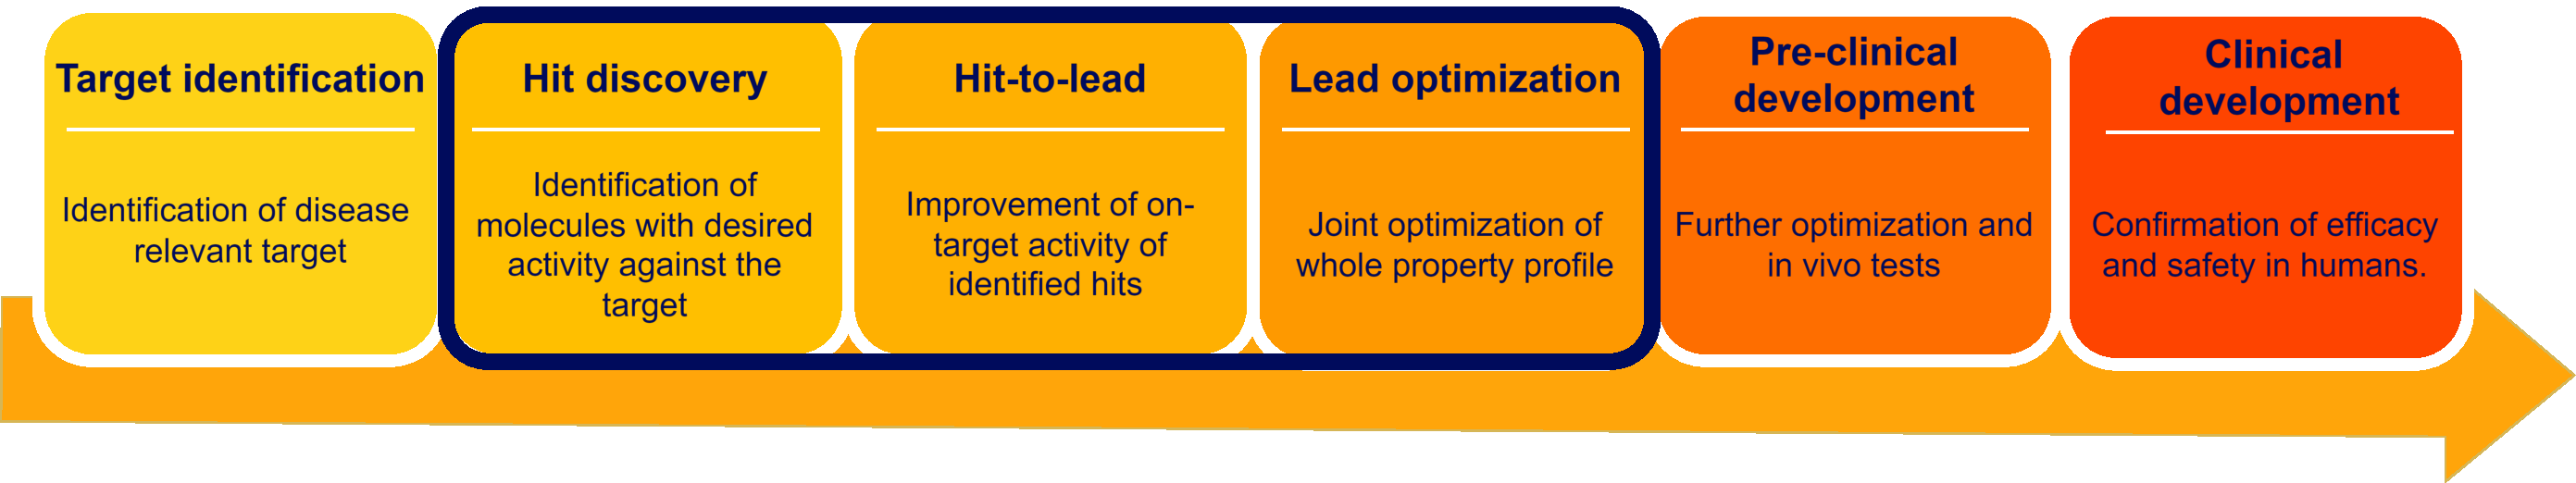
\includegraphics[width=\textwidth]{figures/drug-discovery-pipeline.pdf}
    \caption{The drug discovery pipeline start with the identification of a
    biological target. Once a target is identified, readily available molecules
    are screened for their activity against the target in high-throughput
    screening. Promising hits are then modified and optimized to lead compounds.
    These lead compounds are then further optimized and tested in preclinical.
    Finally, the most promising candidates are tested in clinical trials and
    eventually approved by regulatory agencies. The stages in the blue box are
    highly amenable to machine learning and computational methods and are the
    focus of this thesis. \label{fig:drug-discovery-pipeline}}
\end{figure}
\begin{itemize}
    \item \textbf{Target identification:} The first stage is target identification, 
    where a biological target is identified that is hypothesized to be associated
    with a disease phenotype.
    \item \textbf{Hit discovery:} In the hit discovery stage molecules are
    screened for their activity against the target in high-throughput screening (HTS).
    These lab experiments ,often referred to as assays, are used to measure the
    activity of the molecules against the target in vitro. HTS is resource
    intensive and time-consuming.
    \item \textbf{Hit-to-lead:} Promising hits are then modified and optimized
    to lead compounds. In this stage, the optimization is primarily focused on
    improving the activity of the molecule against the target. This is usually 
    done in a DMTA (Design-Make-Test-Analyze) cycle, where the molecule is
    designed, synthesized, tested in vitro. The results are then analyzed and the cycle 
    continues until a satisfactory lead compound is found.
    \item \textbf{Lead optimization:} The lead compounds are then further
    optimized to improve their properties, such as pharmacokinetics, toxicity or
    specificity. This is usually done in a DMTA cycle as in the
    hit-to-lead stage and also involves the synthesis and testing of the
    molecules in vitro.
    \item \textbf{Preclinical development:} The most promising candidates are then tested in
    preclinical studies. These studies are usually done in animals and are used
    to assess the safety and efficacy of the drug candidate in vivo. 
    \item \textbf{Clinical trials:} Finally, the candidates that pass the
    preclinical studies are tested in humans in clinical trials. 
    These are usually divided into three phases, where the safety and efficacy
    of the drug are tested in increasing numbers of patients. 
    Phase I trials are mainly focused on the safety of the drug, Phase II trials
    are focused on the efficacy of the drug and Phase III trials are focused on
    the safety and efficacy of the drug in a larger population.
    \item \textbf{Regulatory approval:} The final stage is the regulatory
    approval, where the drug is approved by regulatory agencies such as the FDA
    in the US or the EMA in Europe. 
\end{itemize}

The hit discovery, hit-to-lead and lead optimization (blue box in
\Cref{fig:drug-discovery-pipeline}) are highly amenable to machine learning and
computational methods and are the focus of this thesis. Specifically 
we will focus on generative models for molecules, which can help to 
find hits in the hit discovery stage and optimize lead compounds in the
hit-to-lead and lead optimization stages. Furthermore we will look at 
computer-aided synthesis planning (CASP) tools, which can help to find
synthesis routes for promising molecules in the hit discovery and hit-to-lead and lead optimization
stages.

\section{De Novo Molecule Design\label{sec:denovo}}
\subsection{Background}
Goal-directed molecule generators aim to address the challenge of finding novel
molecular structures satisfying a property profile of interest. These property
profiles can include a range of properties, including the activity against a
target, or other important traits such as solubility or toxicity. Given a
computational scoring function that encodes the relevant properties, generative
models operate in a feedback loop, where the scoring function guides the
generation of molecular structures. This contrasts with the traditional approach
of virtual screening \citep{todo}, where a fixed virtual library of molecules is
searched in a brute-force manner. This simple way of searching the chemical
space is inefficient and is not able to tap into the possibilities provided by
the vastness of drug-like chemical space, which is estimated to contain between
$10^{23}$-$10^{60}$ molecules. Generative models, on the other hand, hold the
promise of being able to search chemical space more efficiently and come up with
promising drug candidates.

Triggered by advances in deep learning, the field of generative models for
molecules has seen a surge in interest in recent years. The first deep-learning
based generative models for molecules were based on recurrent neural networks
(RNNs) originally proposed for text generation. After this early work by
\citep{seglerGeneratingFocusedMolecule2018} and
\citep{gomez-bombarelliAutomaticChemicalDesign2018} a great number of different
models have been published
\citep{eltonDeepLearningMolecular2019,sanchez-lengelingInverseMolecularDesign2018}.
These models are based on a large variety of architectures and training
strategies, including autoregressive models, generative adversarial networks
(GANs), variational autoencoders (VAEs), flow-based models
\citep{madhawaGraphNVPInvertibleFlow2019}. One key design choice is the
representation of the molecules, which can be based on SMILES strings,
graph-based representations or 3D structures
\citep{eltonDeepLearningMolecular2019,sanchez-lengelingInverseMolecularDesign2018,pangDeepGenerativeModels2024}.

Generative models are often divided into two categories: \emph{goal-directed}
and \emph{distribution-learning} models. Distribution-learning models learn
general structural patterns in molecules and aim to sample novel molecules that
the training data in distribution. These models are then most often used as a
base for goal-directed models, which aim to find molecules that satisfy a
property profile of interest. These properties are usually encoded in a
scoring function, which is then used to guide the generation process, in a
reinforcement learning style feedback loop.

% The evaluation of generative models is challenging. 
While generative models have shown great promise in generating stable chemical
structures their evaluation is often challenging. While evaluation in
discriminative tasks is usually a straightforward evaluation on a hold-out test
set, the evaluation of generative models requires more complex evaluation
schemes and require to take into account various aspects of the generated
molecules. This has led to the development of a range of evaluation metrics
\citep{preuerFrechetChemNetDistance2018,gaoSynthesizabilityMoleculesProposed2020}
and benchmarks for generative models
\citep{polykovskiyMolecularSetsMOSES2020,brownGuacaMolBenchmarkingModels2019}.
However, the evaluation of generative models is still an active area of research
and challenges remain. In this thesis, we address some of these challenges which
are outlined in the following sections.

\subsection{Evaluation of Distribution-Learning Models}
The evaluation of distribution-learning methods has posed challenges in
different applications, apart from the generation of molecules. While so called
\emph{likelihood-based} models, such as autoregressive models or flow-based
models, can be evaluated using metrics like the negative log-likelihood or
perplexity evaluated on a hold-out test set, other models such as generative
adversarial networks (GANs) \citep{goodfellowGenerativeAdversarialNetworks2014}
do not offer the possibility of this a straightforward evaluation. To this end
alternative metrics have been proposed, spawning its own subfield of research
\citep{heuselGANsTrainedTwo2017}.

In the field of cheminformatics new metrics have been proposed to evaluate the
quality of generated molecules and how well they match the training data in
distribution \citep{preuerFrechetChemNetDistance2018}.
\citet{polykovskiyMolecularSetsMOSES2020} and
\citet{brownGuacaMolBenchmarkingModels2019} introduced the Moses and GuacaMol
benchmarks respectively, which evaluate the quality of generated molecules using
a combination of metrics. Among these are the FCD metric
\citep{preuerFrechetChemNetDistance2018}, the internal diversity
\citep{benhendaChemGANChallengeDrug2017} of the generated molecules, or the
KL-divergence between the distributions of chemico-physical properties of the
generated molecules and the training data.

It is however not clear how informative these metrics actually are and how well
they correlate with the actual usefulness of the tested generative models.

% The early stages of the drug discovery pipeline, including hit discovery,
% hit-to-lead, and lead optimization, heavily rely on experimental screening of
% molecules in wet lab assays to identify promising candidates for further
% development. However, these are resource intensive and the number 
% of molecules that can be tested is limited. Computational methods can help to
% prioritize which molecules to test next, to avoid wasting resources on
% unpromising compounds.

% Virtual screening is a widely used computational approach, in which 
% virtual libraries of molecules are screened in silico to identify promising
% candidates for experimental testing. 



% This traditional approach,
% known as high-throughput screening (HTS), involves physically testing a vast
% number of compounds in specialized assays to identify promising hits and lead
% candidates. However, HTS is a resource-intensive and time-consuming process,
% often involving the synthesis and testing of millions of molecules. To address
% these challenges, computational approaches, collectively termed virtual
% screening, have gained significant traction in drug discovery. Virtual screening
% involves computationally evaluating large libraries of molecules, typically
% using predictive models or simulations, to prioritize the most promising
% candidates for experimental testing. This approach allows for the rapid
% evaluation of vast chemical spaces, reducing the number of molecules that need
% to be synthesized and tested in the laboratory. One widely used virtual
% screening method is structure-based drug design, which leverages the known
% three-dimensional structure of the target protein. In this approach,
% computational docking algorithms are employed to predict the binding affinity
% and pose of small molecules within the target's binding site. Molecules with
% favorable predicted binding modes and energies are then prioritized for
% experimental validation. Another approach, known as ligand-based drug design,
% relies on the knowledge of known active and inactive compounds targeting the
% protein of interest. Machine learning models, such as quantitative
% structure-activity relationship (QSAR) models, are trained on these datasets to
% learn the relationships between molecular structures and their corresponding
% bioactivities. These models can then be used to predict the activity of new
% molecules, guiding the prioritization process.




% \citep{todo}.

% \subsubsection{Prediction of molecular properties and virtual screening}
% Machine learning has shown great promise in accelerating the drug discovery
% process. In the context of small molecule drug discovery, machine learning
% methods have been used to predict a range of properties of interest, including
% the activity of a molecule against a target, its pharmacokinetic properties, its
% toxicity or its synthetic accessibility. These predictions can be used to
% prioritize which molecules to test next, to avoid wasting resources on
% unpromising compounds.


% Why is diversity important?
The diversity of the generated molecules is an important aspect in the
application of goal-directed generative models. Given that the scoring functions
are usually only an imperfect and incomplete approximation of the desired
properties, finding a diverse set of molecules that score well can increase the
success chancess of downstream stages of the drug discovery project. Given the
expected failure of some of the candidates in later experiments, having a backup
of other candidates with somewhat different structure can be beneficial.

It is unclear how well current generative models perform in generating diverse
high-scoring molecules, which is due to a combination of two main factors. 
Firstly, many commonly used diversity metrics are inadequate for evaluating
diverse optimization approaches. This results in uninformative benchmarks that
do not meaningfully measure the diversity of the generated molecules. Secondly,
a meaningful comparison of goal-directed generators necessitates a standardized
compute budget. This is because the performance of generative models depends strongly 
on the amount of ressources available for training and evaluation.

\subsection{Evaluation of Goal-Directed Generators}
In goal-directed generation tasks, the generative models are tasked to find
molecules with high scores according to a scoring function that encodes the
desired properties of the generated molecules. The scoring functions used in
these tasks are often based on ML models trained on experimental
data. This can lead to problems, as the optimization process can overfit to
biases of these ML models. 

It is a well-known problem in generative modelling that the optimizing the
output of classification/regression models with respect to their inputs can lead
to unsatisfactory results \citep{todo}. In the context of goal-directed molecule
generators we identified two possible failure modes: Firstly, the generative
models can overfit to artifacts of the scoring function, which are not actually
relevant for the properties of interest. Secondly, the generative models may
overfit to the training samples used to train the scoring function, which can
lead to a lack of novelty in the generated molecules.

\section{Retrosynthesis Prediction\label{sec:retrosynthesis}}
% Retrosynthesis planning is important and ML can help
Drug candidates, whether suggested by generative models or found by other means,
at some point need to be synthesized in for further testing and 
eventually for use in patients. The synthesis of a molecule is usually a complex
process, involving multiple steps of chemical reactions. Computer-aided synthesis 
planning (CASP) can help by finding new synthesis routes for a target molecule.
In some cases, this can lead to more efficient and cheaper synthesis routes, or
even enables the synthesis of previously inaccessible molecules.

% Synthesis planning 
The most popular approach to CASP is retrosynthesis planning. Starting from a
target molecule, the goal is to predict a chain of chemical reactions that can
transform readily available starting materials into the target molecule. This
problem is usually formulated as a graph search problem, where the nodes are
molecules and the edges are chemical reactions. The goal is to find a path from
the target molecule to a set of starting materials, which can be synthesized in
the laboratory. The connectivity of this graph is given by retrosynthesis
prediction models, which given a target product, predict which reactants it can
be made from. Highly accurate retrosynthesis prediction models are necessary for
the success of CASP tools, as otherwise the suggested synthesis routes might not
be feasible in the laboratory.

% A prominent approach to CASP is template-based planning
% Mention transformers and graph-based models
Template-based models are a popular approach to retrosynthesis prediction. These
models use so called reaction templates, which are graph transformation rules 
that encode connectivity changes between atoms during a chemical reaction. These 
templates can be either automatically extracted from a reaction database or
hand-coded by a chemist. Given a target molecule, the goal is then reframed as a
classification task, where the model predicts which templates can be used to
synthesize the target. Application of the graph transformation rules then leads
to reactants that can be used to synthesize the target molecule. While popular, 
these models have some limitations, in common datasets many templates only occur 
in few training samples, which makes it difficult to train a model that generalizes
well for these rare templates.

In \citep{seidlImprovingFewZeroShot2022} we study the problem of single-step
retrosynthesis prediction. Given a target molecule, the goal is to predict a
set of reactants that can be used to synthesize the target molecule.
Template-based models are a popular approach to single-step retrosynthesis
prediction. These models use so called reaction templates, which are
either extracted from a reaction database or hand-coded by a chemist.
Given a target molecule, the goal is then reframed as a classification task,
where the model predicts which templates can be used to synthesize the target.



\section{Aims and Objectives}
\subsection{Highlighting Failure Modes in Evaluating Generative Models}
In \citep{renzFailureModesMolecule2019} (\cref{sec:failure-modes}) we show the
limitations of the GuacaMol distribution-learning benchmark, by evaluating the
performance of different sophisticated generative models on this benchmark, and
comparing it to a simple baseline model that generates molecules by introducing
minor variations of the molecules in the training data. We show that the 
most of the tested generative models do not outperform the simple baseline
model, or only do so marginally. This suggests that the tested benchmarks
are not be able to distinguish state-of-the-art generative models 
from simple baseline models, and call for a more comprehensive evaluation of
distribution-learning models. \Cref{sec:failure-modes} reprints
the corresponding publication.

In \citep{renzFailureModesMolecule2019} we introduce \emph{control scores} that
give information whether the optimization overfits to artifacts of the scoring
functions, or the training data. We do this by training additional scoring
functions, trained with either a different random initialization or trained on a
hold-out subset of the the available training data. Using this approach, we can
show that generative models overfit to the scoring function's random
initialization and to high-scoring training samples. This shows that the reported
performance of these models is an overestimation, and that our control 
scores can be used to obtain a more meaningful evaluation of goal-directed 
molecule generators. \Cref{sec:failure-modes} reprints
the corresponding publication.

\subsection{Diversity-based benchmark of Goal-Directed Generators\label{sec:divopt}}
In \citep{renzBenchmarkingEfficiencyGenerative2024} we introduce a benchmark for
diverse optimization that addresses the above-mentioned issues. In this
benchmark, we evaluate the diversity of the generated molecules using a recently
proposed diversity metric \#Circles \citep{xieHowMuchSpace2023}. We compare the
performance of diverse optimization approaches under two different compute
budgets, namely a fixed number of scoring function evaluations and a fixed time
budget. The first setting is relevant for applications where the cost of
evaluating the scoring function dominates the optimization process, while the
second setting is relevant for scoring functions that are cheap to evaluate.
Using this setup we test 14 goal-directed optimization methods and show how
SMILES-based auto-regressive models dominate the benchmark.
\Cref{sec:diverse-efficiency} reprints the corresponding publication.

\subsection{Improving Few-Shot and Zero-Shot Retrosynthesis Prediction}
In \citep{seidlImprovingFewZeroShot2022} we propose a novel approach to
template-based retrosynthesis prediction. We use a multimodal learning approach
that learns to associate relevant templates to product molecules using a Modern
Hopfield Network \citep{ramsauerHopfieldNetworksAll2020}. Our model can leverage
structural information about the templates and can make use of similarities
between them. This allows for improved generalization, especially for templates
with few training samples and even for unseen templates. This model is several
times faster than comparable methods and shows good predictive performance.
\Cref{sec:mhn-react} reprints the corresponding publication.

\section{List of Publications\label{sec:publications}}
This thesis comprises the work published in the following papers:

\begin{itemize}
    \item \fullcite{renzFailureModesMolecule2019}
    \item \fullcite{renzBenchmarkingEfficiencyGenerative2024}
    \item \fullcite{seidlImprovingFewZeroShot2022}
\end{itemize}



% give overview over my other publications
\paragraph{Other Publications} Besides the papers listed above, I have also
contributed to the following publications:

\begin{itemize}
    \item \fullcite{preuerFrechetChemNetDistance2018}
    \item \fullcite{renzUncertaintyEstimationMethods2019}
    \item \fullcite{hofmarcherLargescaleLigandbasedVirtual2020}
    \item \fullcite{renzLowCountTimeSeries2023}
\end{itemize}